\chapter{Tic-tac-toe}
\label{chap:ttt}

\section{Motivation}

After the familiarization with pyProCT code, execution flow and parameters it is time to analyze it's performance and better understand the scheduler implementation. I developed an small program designed to test the scheduler, learn to use the analysis tools, such as Paraver, find possible problems that may arise due to the parallelization, like the reproducibility on random algorithms or the results validation, and, in general, use all the required tools on a smaller scale than pyProCT. 

The developed program was an command-line implementation of the popular game Tic-tac-toe. It suited quite well the project needs because it featured good parallelization options, stochastic elements, a clear turn structure (easing up the first analysis trials), variable-size parametrized tasks and automatized execution (having two AI playing).

\section{Execution Flow}

\hyperref[fig:tic-tac-toe]{Figure \ref{fig:tic-tac-toe}} shows a simplified version of the program's execution flow. All the logic handling which player's turn is, how the board is marked and some other parts have been omitted because they are not relevant. 

For each turn, while the game is not finished, the program calls the player's play function. The algorithm implementing the AI moves is a montecarlo-like method, it randomly simulates a big number of games for each available cell and then choses the cell with the best score.

To do this it first gets all the free cells, then for each available one it calls the exploration\_handler method. This method in turn calls mark\_an\_explore a number of times (this number is defined by the ITERATIONS parameter which is a command-line argument) with a copy of the game board. Basically, mark\_and\_explore first the cell passed as parameter and then fills randomly the copied board, till the game is finished (either by a player winning or a draw), returning the cell and the id of the winning player or a 0 if there is a draw. The list of winnig id's is then returned to the montecarlo function. Afterwards we initialize the score value for each available cell with infinity. Then for each tuple containing a cell and the winner of that simulation we increment the the score of the cell if the player has won or decrease it if the player has lost (the algorithm could modify the score for draw results), the actual increment/decrement values can be tuned but for testing purposes it's not relevant. 

\section{pyScheduler refactor}

Once the sequential program was ready, the next step was to decide how to refactor it to use pyScheduler \footnote{https://pypi.python.org/pypi/pyScheduler/0.1.0}, which the current scheduler used by pyProCT. The decision was to consider each exploration\_handler as a task because it would be interesting to see how task's size affects the performance of the scheduler and, having the ITERATIONS parameter to change the number of iterations performed inside the exploration\_handler, this was deemed the best option. 

The selected scheduler has three scheduling types, one sequential and two parallel: 

\begin{description}
\item [Serial,] which executes the task sequentially.
\item [ProcessParallelScheduler,] which uses python's multiprocessing module.
\item [MPIParallelScheduler,] which uses mpi4py for the parallelization.
\end{description}

The usage of the scheduler is simple. For each task we have to call the \textit{add\_task} method providing the following information:

\begin{description}
\item [Task name:] a unique task name.
\item [Dependencies:] a list of this task dependencies (which must be a list of other tasks names).
\item [Description:] a description of the task.
\item [Target function:] the name of the function to be executed.
\item [Function kwargs:] the list of the keyword arguments which need to be passed to the target function.
\end{description}

Once the task list is completed we just need to call the run() method of the scheduler. The method will return a list with the execution results of each task.

For the tic-tac-toe these are the values for the queued tasks:

\begin{description}
\item [Task name:] ExplorationXY (being X, Y the coordinates of the cell to be explored).
\item [Dependencies:] [ ] (the empty list because there are no dependencies among different explorations).
\item [Description:] Montecarlo exploration.
\item [Target function:] self.exploration\_handler (as we are inside Player class namespace we must add the self).
\item [Function kwargs:] {"x": x, "y": y, "board": board} (being X, Y the coordinates of the cell to be explored, and board the current state of the game).
\end{description}

\section{Instrumenting with Extrae}

Next step was to start using the analysis tools. The decision was to use the  \textbf{Extrae + Paraver} combination. Extrae \footnote{http://www.bsc.es/computer-sciences/extrae} is the package used for instrumenting the code; paraver \footnote{http://www.bsc.es/computer-sciences/performance-tools/paraver} is the tool used to visualize the traces generated by Extrae. These tools have been both developed at the BSC to be used together. We chose them because of the Extrae support to python, the offered assistance and proximity of the tools' experts and the fact that they are both installed and configured on MareNostrum III, which is our target execution platform.

Extrae offers two different ways to instrument the code: automatically instrument functions (providing a list of functions to the extrae XML configuration file) or including the extrae module (import pyextrae)  and emit specific events inside the code with \textit{pyextrae.eventandcounters(type, value)}. 

The basic usage of the first, which  does not require any changes on the code, instruments the entry and exit points of the functions; more complex behaviours are also available but for these tests the basic one is enough. 

The second one just needs to add the mentioned function call wherever we are interested to emit an event.

To start, I set \textit{play, montecarlo} and \textit{exploration\_handler} methods to be automatically instrumented and added a two events: one before the scheduler intialization and task addition and one just after the scheduler run(); on the sequential version \footnote{ From now, "sequential" will refer to the schedulerless version, "serial" to the one with the serial scheduler, "parallel" for the one using ProcessParallel and "mpi" for the mpi4py one} this corresponds to before and after looping through the available cells (calling \textit{exploration\_handler} on each iteration).

Support for python is only available from version 3.0 onwards and it's not fully tested so we faced some problems. For the sequential and serial versions everything went well, the traces  were correct and they could be visualized with Paraver. For the parallel version we were not able to extract correct traces as extrae was not able to detect the parallelization method. When I tried the MPI version it didn't work either for two reasons. On one hand, adding the user functions' automatic instrumentation made the whole execution to end with a segmentation fault without generation the traces. On the other hand, using just the event emit method, the visualization showed just one thread. 

After meeting with BSC people we managed to solve the issue. The problem was that extrae used a sequential-tracing library, so it could not detect the mpi multiple threads. To solve it we substituted this sequential library with an mpi-tracing one. After some work on their part the first issue was also solved by changing some values on \textit{Extrae\_define\_event\_type}. 

For the parallel implementation with multiprocessing this approach wasn't supported. They gave me some ideas to try but to no avail. I linked extrae with a number of different libraries, such as the pthreads one, to see it they were able to hook themselves to the python multiprocessing threads but it didn't work. I left the issue open and went forward. Fortunately, after working on the new tracing system for pyCOMPSs at the BSC, I managed to develop a workaround tracing system albeit quite more rudimentary and inconvenient to use. Extrae has a command line usage of which I used two basic commands:

\textit{extrae-cmd init node slots}

\textit{extrae-cmd emit slot event\_value event\_type}, 

I created a Python class wrapper for this two commands. This way I reused it to instrument the pyProCT later. This class deals with the extrae paths, concurrency as well as providing a easier interface to call from python. To use it first it is necessary to initialize each used node with an ID and the number of processes/threads it will contain. Then for each event we want to emit we specify it's ID (which must be positive and smaller than the number of threads we set for that node) and the value and type of the event. 

The first trials I dit raised a segmentation fault; knowing that emitting an event with an out-of-range thread ID raises a segmentation fault I figured out that the initialization was not correct. I tried a number of different methods. Because this extrae usage is not the recomended nor normal approach there is no documentation for it nor examples for it. After several days working on it I resolved to meet with the extrae team. Working with them we found out that the segmentation fault was caused by a bug on the release I was using. Kindly they fixed it and made a custom package for me to use. With it I finally was able to achieve a basic instrumentation for the parallel (with python-multiprocessing) version. This is limited to emit events and can not produce the advanced visualizations and results achieved on the serial and MPI version.

\begin{landscape}
\begin{figure}
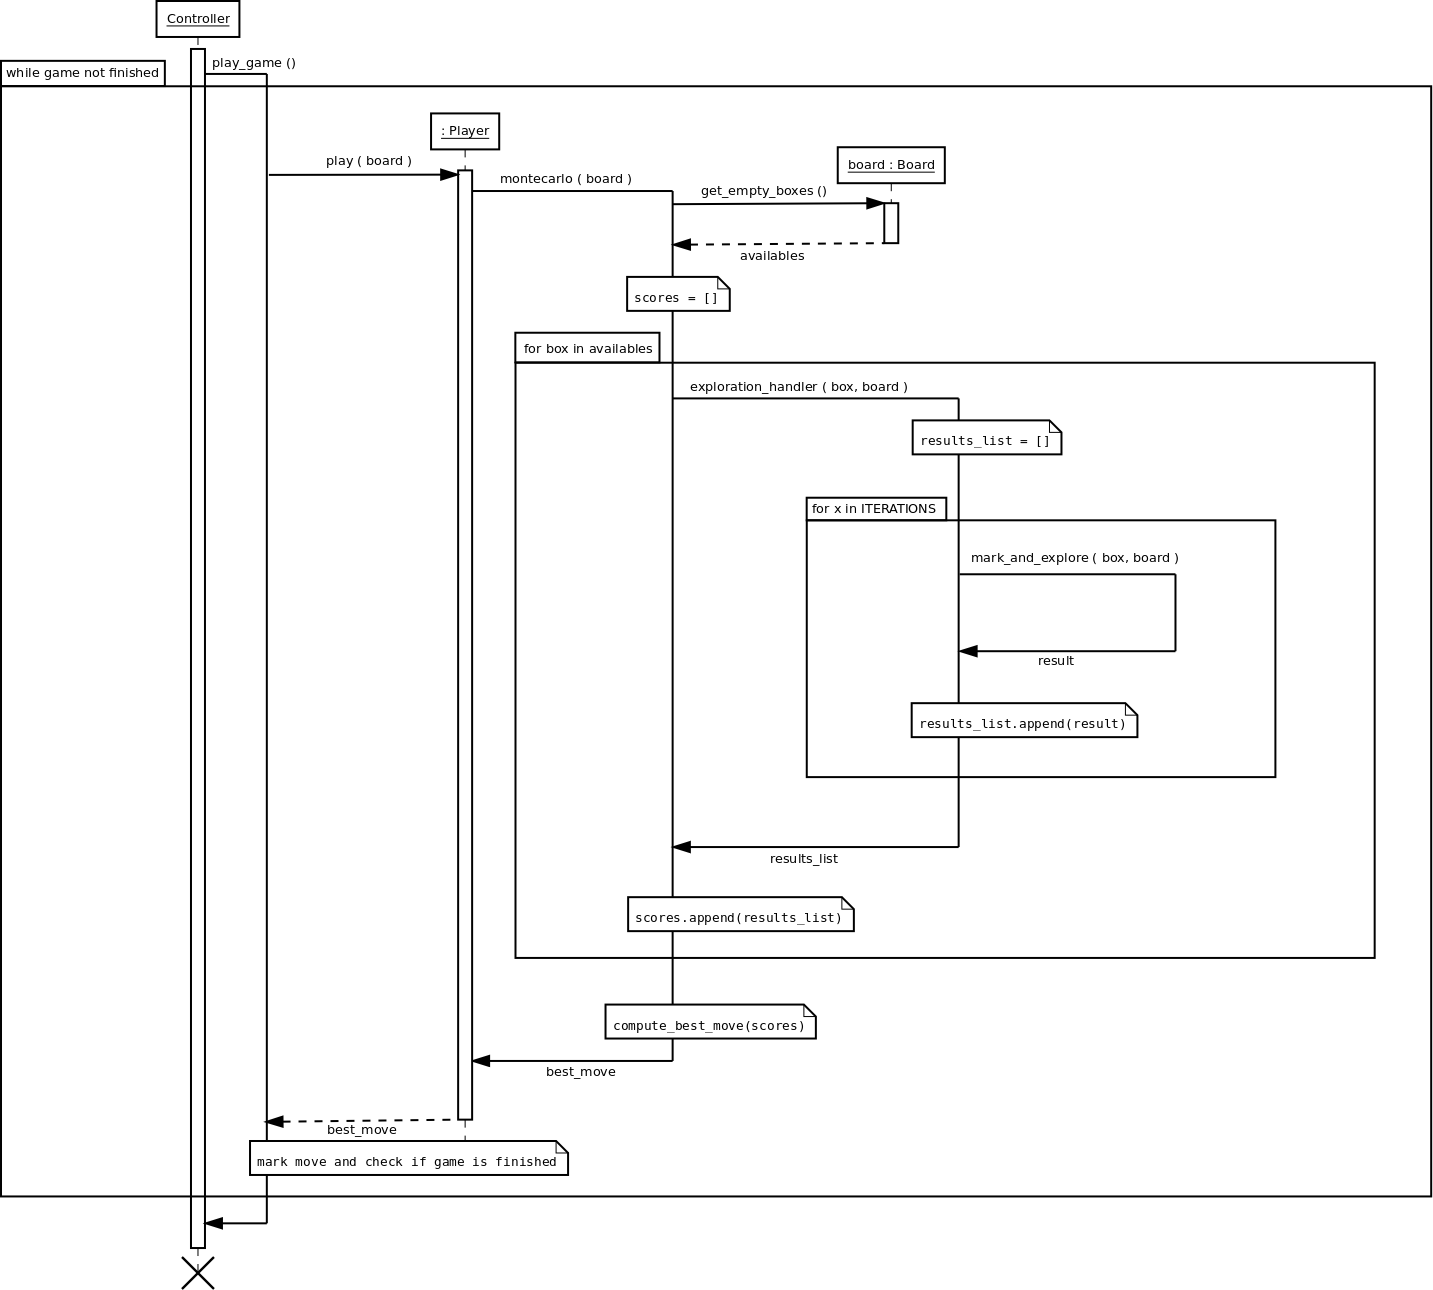
\includegraphics[width=20cm]{img/tic-tac-toe.png}
\caption{Tic-tac-toe Execution Flow}
\label{fig:tic-tac-toe}
\end{figure}
\end{landscape}


\section{Visualizing with Paraver}


Once generated the trace file the next step is to analyze them with the visualization tool Paraver.

First thing was to create a configuration file that would show the instrumented user functions (montecarlo, play and exploration\_handler on this program). To do so I configured the event filter to show only events of the type 60000100 (which is the type assigned to instrumentated user functions), and the semantic options to show the last event value (that is the values identifying the functions) in a stacked composition. Thanks to the ability of copy/paste time info from a graphic we can quickly compare different traces.

 \hyperref[fig:fig:ttt-python-funcs-seq]{Figure \ref{fig:ttt-python-funcs-seq}} shows the visualization of three executions of the tic-tac-toe, all of them with 500 iterations. The first is an schedulerless version, the second with the serial scheduler and the last one with an MPI scheduler. At the time of writing the parallel/multithreading scheduler can't be instrumented, as this is a demo section of the Paraver capabilities we have considered that leaving the parallel version out will not harm the purpose of this section. Dark blue corresponds with exploration\_handler function, white with montecarlo, red with play and light blue the time outside these three functions; the MPI version has more labels but for the current section the details aren't important. We can see on the figure that the serial scheduler has an important overhead, making it slower than the schedulerless version, but the MPI scheduler is quite faster.
 
 
\begin{figure}[h]
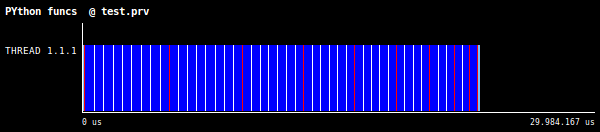
\includegraphics[width=\textwidth]{img/ttt_500_python_funcsG11.png}
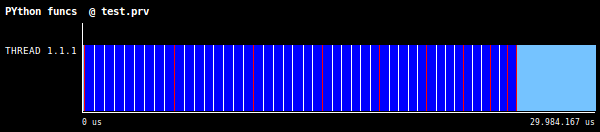
\includegraphics[width=\textwidth]{img/ttt_500_python_funcsG12.png}
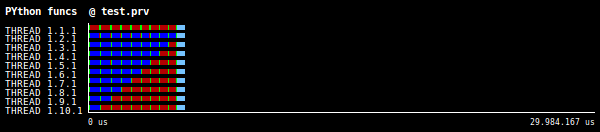
\includegraphics[width=\textwidth]{img/ttt_500_python_funcsG13.png}
\caption{Tic-tac-toe 500 iterations executions}
\label{fig:ttt-python-funcs-seq}
\end{figure}


Paraver has a wide range of configurations to visualize MPI information (see \hyperref[fig:fig:ttt-mpi-IPC]{Figure \ref{fig:ttt-mpi}} ), useful execution time or IPC. We can inspect data in timeline or tabular form but also with the aid of other tools such as the Clustering. With this tool we can cluster the results to obtain, for example, a graphic relating the executed instructions and the IPC. Thanks to this we can bypass analysis problems related with the time where, sometimes, an increase or unbalance in the workload depends on the IPC rather than the number of instructions. On \hyperref[fig:fig:ttt-mpi-IPC]{Figure \ref{fig:ttt-mpi-IPC}} we can see that the most computation-intensive areas associated with the exploration\_handler function (in blue on  \hyperref[fig:ttt-python-funcs-seq]{Figure \ref{fig:ttt-python-funcs-seq}}) have a good efficiency. 
 
 
\begin{figure}[h]
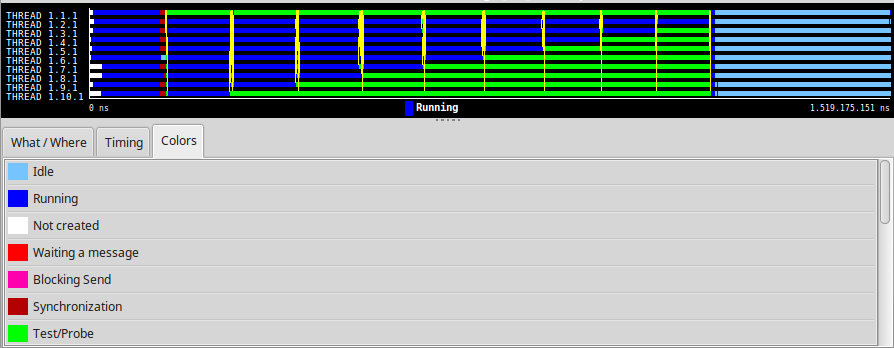
\includegraphics[width=\textwidth]{img/New_window_1_2DZoom_range_[1,6]@test.png}
\caption{Tic-tac-toe MPI information for a 500 iteration execution}
\label{fig:ttt-mpi}
\end{figure}


 
\begin{figure}[h]
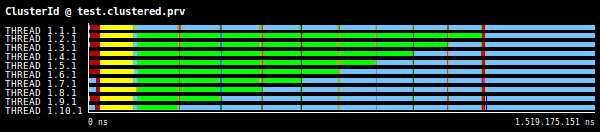
\includegraphics[width=\textwidth]{img/cluster_graph_mpi.png}
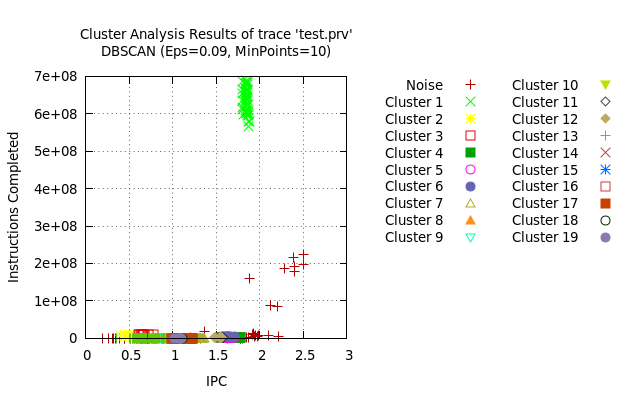
\includegraphics[width=\textwidth]{img/cluster_mpi_IPC.png}
\caption{Tic-tac-toe timeline and clustering for 500 iteration MPI execution}
\label{fig:ttt-mpi-IPC}
\end{figure}



